\subsection{Application plan}
The application that implements the proposed pitch detection system will take the form of a graphical web based application. The web is chosen for portability and ease of use. The end user, be it an individual wanting to learn to sing or a choir testing candidates, can use any mobile device with a microphone, be it a laptop, tablet or smartphone, and without installing anything test the accuracy of their singing or tune their guitar.

\subsection{Web Audio API}
As the pitch detector is intended to be used in the browser, for portability and ease of use, the Web Audio API will be extensively used. The purpose of the API is to allow developers controls over audio processing functionality on browsers, by getting access to user audio devices, adding effects and more. 
The Web Audio API operates in a AudioContext, which can be thought of as an empty control flow graph. The graph is constructed using AudioNodes which fall into one of three categories; input or source nodes, modifier nodes and output nodes. The nodes are then connected to each other to form the graph. 

The graph operates by passing blocks of data (called render quanta) between nodes, where one render quantum consists of frames of samples, where one frame contains one sample for every audio channel, at least according to the W3C Audio API 1.1 specifications. Render quantum seems to be a term reserved for the low level processing of the data passing between nodes, and in reality the audio samples are contiguous for each channel. The important thing to realize here is that the blocks of data, which will be called render quanta for a lack of naming at API level, are 128 in length.

%https://www.w3.org/TR/webaudio/#rendering-loop

\subsubsection{Sources and destinations}
The source node, as their names imply are entry points for audio control graph, they provide signals. Some of these include the OscillatorNode, a node which produces pure sinusoids, a MediaElementAudioSourceNode, which uses the media in an existing HTML audio element. As the purpose of the application is for the user to be able to record their own singing and have it analyzed for pitch correctness, the source in this case will be a MediaStreamAudioSourceNode, which provides a source signal from a MediaStream. The actual source will the method navigator.mediaDevices.getUserMedia\(\) that provides the MediaStream, but this is technically outside the AudioContext so it's not a source node.  
The output may be either the user's system's speakers, or another MediaStream. In this case, there won't be an output node because it's simply not needed. The output will be the result of the fourier analysis.

\subsubsection{Modifiers} 
The modifier nodes are the nodes that are neither sources nor destinations, they take in the signal from a node, performs some transform on the signal, and then hands it over to the next node, or nodes, in the graph. Some of these nodes apply effects, like rever or gain, some can be used for visualizing audio, some can be used to split audio into separate channels for per-channel modification.

The available modifiers unfortunately do not help with the development of the pitch detector, so a lot of the processing would be done with Worklet nodes, a node that allows custom functionality. With this in mind, the simplest way is to not use the Audio API audio graph, but to just take the output from the microphone and in the simplest possible way turn it into data to be processed using regular procedural programming. The AnalyserNode has fourier transform capabilities but there does not seem to be a way to zero-pad it, which is integral to achieving both real-time processing and enough frequency resolution for base singers. 

\subsection{Pitch detector architecture}
The identified steps of the pitch detector at the highest level are recording, zero-padding, FFT, peak picking and some post processing. It's a simple pipeline of collecting enough samples for the FFT from a microphone and then running analysis on the spectrum data. The only problem at this stage is converting the stream from the microphone to something that can be processed. There seems to be mainly two ways to go about implementing this kind of conversion. One way is to feed the stream from the microphone into a recorder and decoding the binary data that becomes available with time. The other is to build a custom audio processor that handles the processing, whatever that may be. 

As the fourier transform and any peak picking algorithm of choice works in the frequency-domain, using the audio graph doesn't make much sense. The only thing the audio graph would be responsible for would be moving the render quanta between processors, but this is a bit like using a chainsaw to slice bread. Figure \ref{fig:pdArch} shows the proposed architecture which uses a bridge node to send the raw audio data from the audio rendering thread to the main thread. For every render quanta processed the data is passed through the node-processor port from the processor to the node in the main thread where it's passed from the node to a callback function. This callback function may then be used to accumulate the render quanta start analysis.

\begin{figure}[ht]
    \centering
    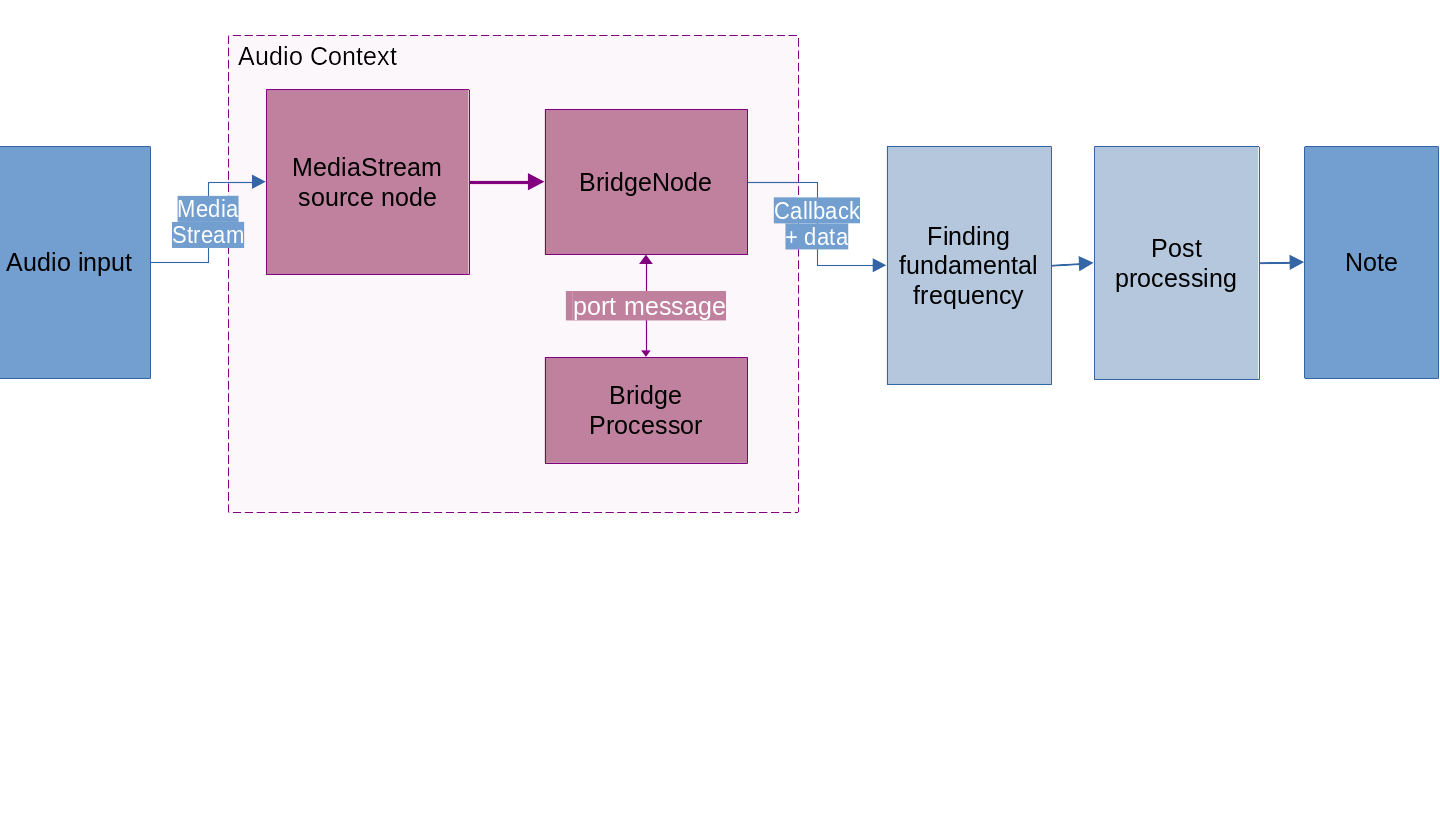
\includegraphics[width=\textwidth]{./images/pdArchitecture.png}
    \caption{Architecture describing the pitch detector. Stream is converted to a data array by having a worklet node send the raw audio data through the node-processor port to be used on the main thread.\label{fig:pdArch}}
\end{figure}

The proposed architecture offers flexibility without being overly complicated. The audio graph may be used to change the input from a microphone to a recording for validation/testing. It would also be possible to apply a real-time time-domain low-pass filter between the input node and the bridge node which would allow downsampling and thus smaller FFT windows if computational power is a constraint. 

\subsection{Implementing the pitch detector}
With a plan for the application, the next step is to implement it. The implementation, based on the arhictecture can be be roughly divided into 4 parts: recording or otherwise taking an input, passing data between the threads, accumulating and performing analysis.
\subsubsection{Audio input}
As the application is to utilize the audio graph, any one of the source nodes may be used to input data into the pitch detector. For development, a reliable source signal is of more value than my sad attempt at singing, so a series of mp3 files, some of which were provided by Finlands svenska manssångarförbund (FSM), an alliance of finland-swedish men's choirs were used using a MediaElementAudioSourceNode. The mp3 files provided by FSM were for some reason set up so that the dominant voice is alone on channel and the 3 others are on the other stereo channel. This is no problem for the audio node based application, we can simply put a channel splitting node between the source node and the detector bridge node.
\lstinputlisting[style=javascript]{../snippets/PitchDetector-B.js}
\subsubsection{Worklet nodes}
Audio worklet nodes are a method of implementing custom audio modifier and sources (a white noise generator for example). In this work, an AudioWorklet node will be used to implement the BridgeNode.

The code snippet below shows how the BridgeNode is implemented.
\lstinputlisting[style=javascript]{../snippets/BridgeNode-A.js}
The bridge node extends or inherits the AudioWorklet node class and methods are added. When the node receives data on its port, it just forwards it to a handler. The handler could do further processing on the data but for the moment only forwards it to the callback function in the pitch detector. The pitch detector callback function is the one responsible for accumulating samples, zero-padding etc.

As the BridgeNode doesn't override or specify anything new, it's really only a thin wrapper for an AudioWorkletNode which is evident by the constructor calling the super constructor, which invokes the parent class constructor. The bridge node is an AudioWorkletNode that uses a BridgeProcessor which also must be created. 
\lstinputlisting[style=javascript]{../snippets/BridgeProcessor-A.js}
As the purpose isn't to actually process anything in the audio context, but rather to utilize the flexibility of the audio graph and have processing done elsewhere, the processor simply sends everything it receives over the port to the corresponding node. 

The only thing left to do is to instantiate a BridgeNode. What connects to it may be a microphone, an audiofile, a gain node, a channel splitter, or anything else that may be useful for the pitch detection.
\lstinputlisting[style=javascript]{../snippets/PitchDetector-A.js}

\subsubsection{Audio processors}

\subsection{Post processing}

\subsubsection{MIDI number to semitone name}
The MIDI number is conveniant because it's a simple integer and a standard. However, for most people, the semitone name means more than the MIDI number. To convert the MIDI number to a semitone, two formulae can be derived using known MIDI numbers and their corresponding notenames. As the semitones repeat every octave and an octave consists of 12 semitones, the index that will be used to find the semitone is computed with modulo 12. The octave number is computed by rounding down the result of the MIDI number divided by 12. For some reason, the MIDI numbers misalign with the octave numbers, C0 being MIDI 12, the octave is shifted down one more step. 
\begin{lstlisting}[style=javascript]
function getSemitoneName(midiNumber) {
    const SEMITONES = ["C", "C#", "D", "D#", "E", "F", "F#", "G", "G#", "A", "B", "H"]

    const letter = SEMITONES[midiNumber % 12];
    const octaveNumber = parseInt(midiNumber/12) -1;

    return "" + letter + octaveNumber; 
}
\end{lstlisting}


\subsection{Integrating with VSS}
VSS is an initialism that will be used to refer to the host application that can compare the pitch detector result to the notes of a piece or song. 
% The big idea:
% source node (microphone) -> % 
% https://developer.mozilla.org/en-US/docs/Web/API/Web_Audio_API
\subsection{The FFT implementation}
% The problem here is that I don't want to be restricted to an FFT window size of a power of 2
% https://github.com/indutny/fft.js/
